\documentclass{standalone}

\usepackage[usenames,dvipsnames]{xcolor}
\usepackage{tikz}
\usepackage{pgfplots}
\usepackage{graphicx}
\usepackage{comment}
\pgfplotsset{compat=1.18}


\pgfplotsset{compat=newest}

\definecolor{Okabe1}{RGB}{000,158,115}
\definecolor{Okabe2}{RGB}{000,114,178}
\definecolor{Okabe3}{RGB}{086,180,233}
\definecolor{Okabe4}{RGB}{230,159,000}
\definecolor{Okabe5}{RGB}{213,094,000}
\definecolor{Okabe6}{RGB}{204,121,167}

\begin{document}
	\vspace{1cm}
		\begin{tikzpicture}
		\begin{axis}[
			enlargelimits=false,
			tick pos=left, %
			tick align=outside, %
			axis line style={opacity=0}, %
			after end axis/.code={
				\draw ({rel axis cs:0,0}
				-|{axis cs:2,0}) % xmin (line starts here)
				-- ({rel axis cs:0,0}
				-|{axis cs:10,0}); % xmax (line stops here)
				\draw ({rel axis cs:0,0}
				|-{axis cs:0,0.6}) % ymin (line starts here)
				-- ({rel axis cs:0,0}
				|-{axis cs:0,1.6}); % ymax (line stops here)
			},
			xlabel={Indent Type},
			ylabel={$k/k_o$},
			xtick = {2, 4, 6, 8, 10},
			xticklabels = {No Indent, Pinch, Side, Cylinder, Point},
			width=10cm,
			xmin=0.5, xmax=11.5,
			ymin=0.6, ymax=1.6,
			scatter/classes={
				%b={mark=*,color=Okabe6},
				c={mark=*,mark size=3pt,color=Okabe3,fill=Okabe3!80,opacity=0.75}
			}
			]
			\addplot[scatter,only marks,% 
			scatter src=explicit symbolic, % Needed for scatter class styling
			error bars/.cd,
			x dir=both, x explicit,
			y dir=both, y explicit
			] 
			table[y error index=2, meta=label] {
				x 	y 		yerr 	label
				2 	1		0.024	c
				4 	1.224	0.191	c
				6 	1.27	0.115	c
				8 	1.298	0.042	c
				10 	1.520	0.045	c	
			};
			\node[anchor=north, inner sep=.5cm] at (axis cs:2, 1) {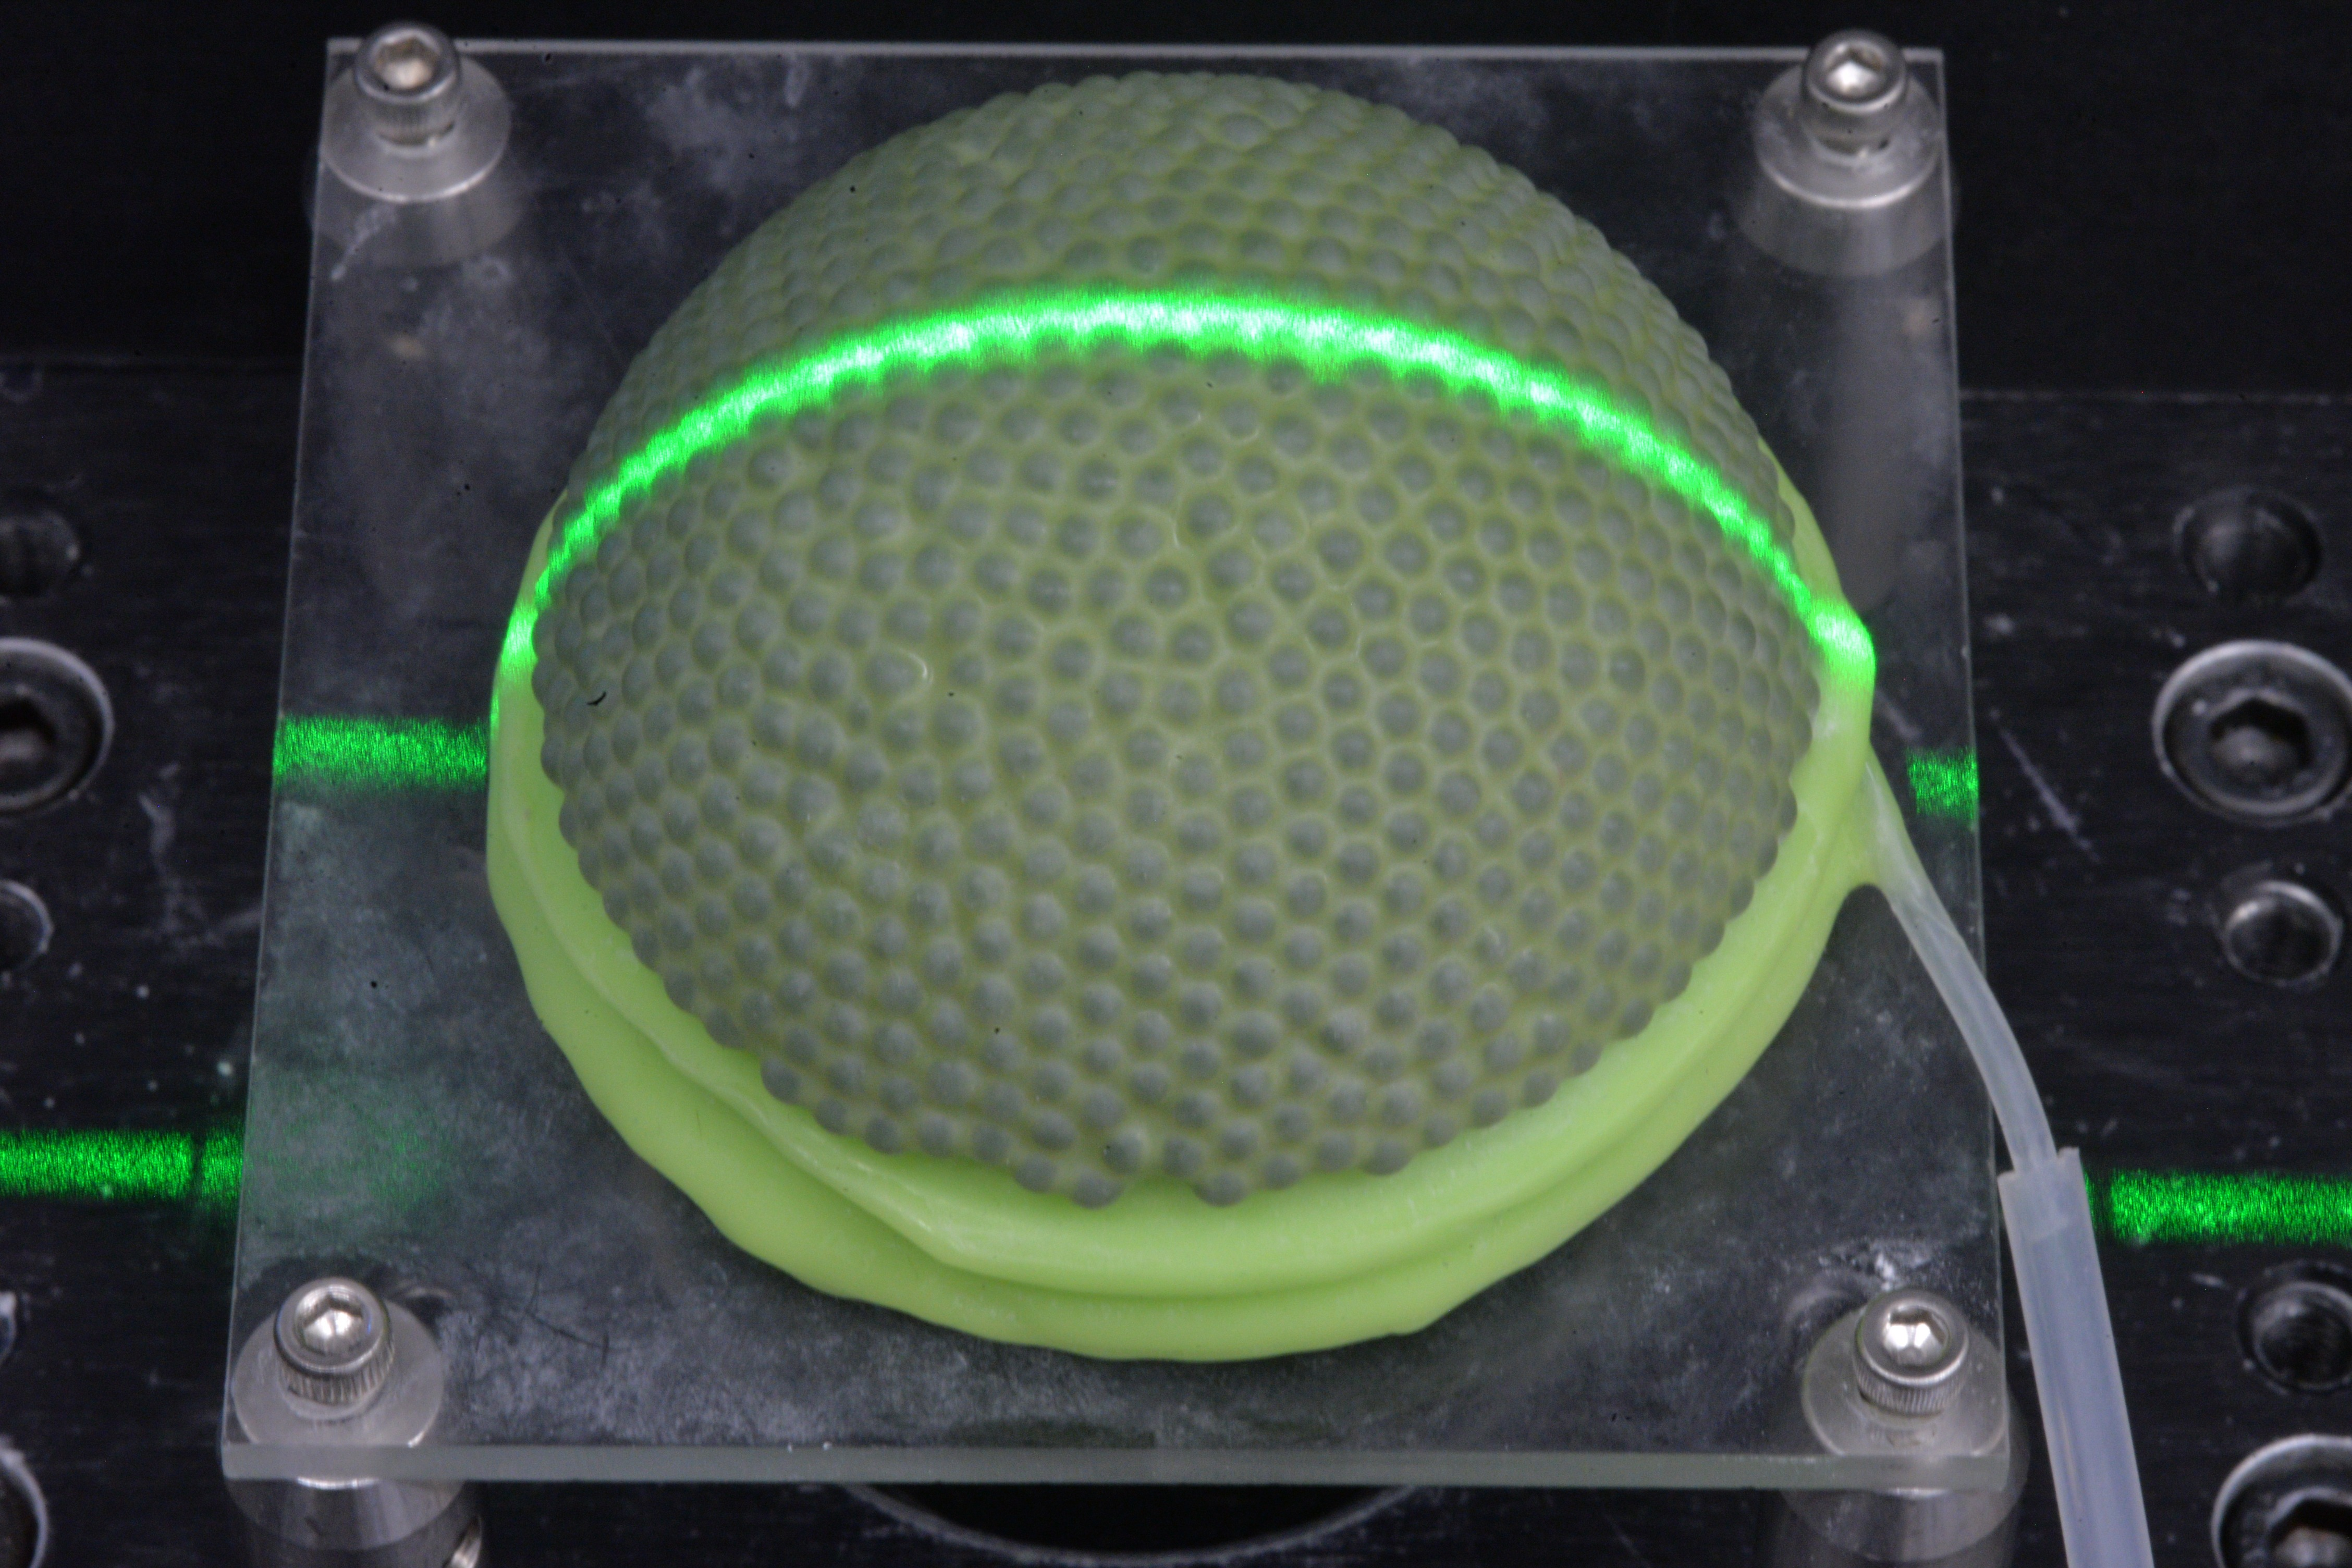
\includegraphics[width=1.5cm, trim= 80 20 120 0,clip]{indent-none}};
			\node[anchor=north, inner sep=1cm] at (axis cs:4, 1.106168525) {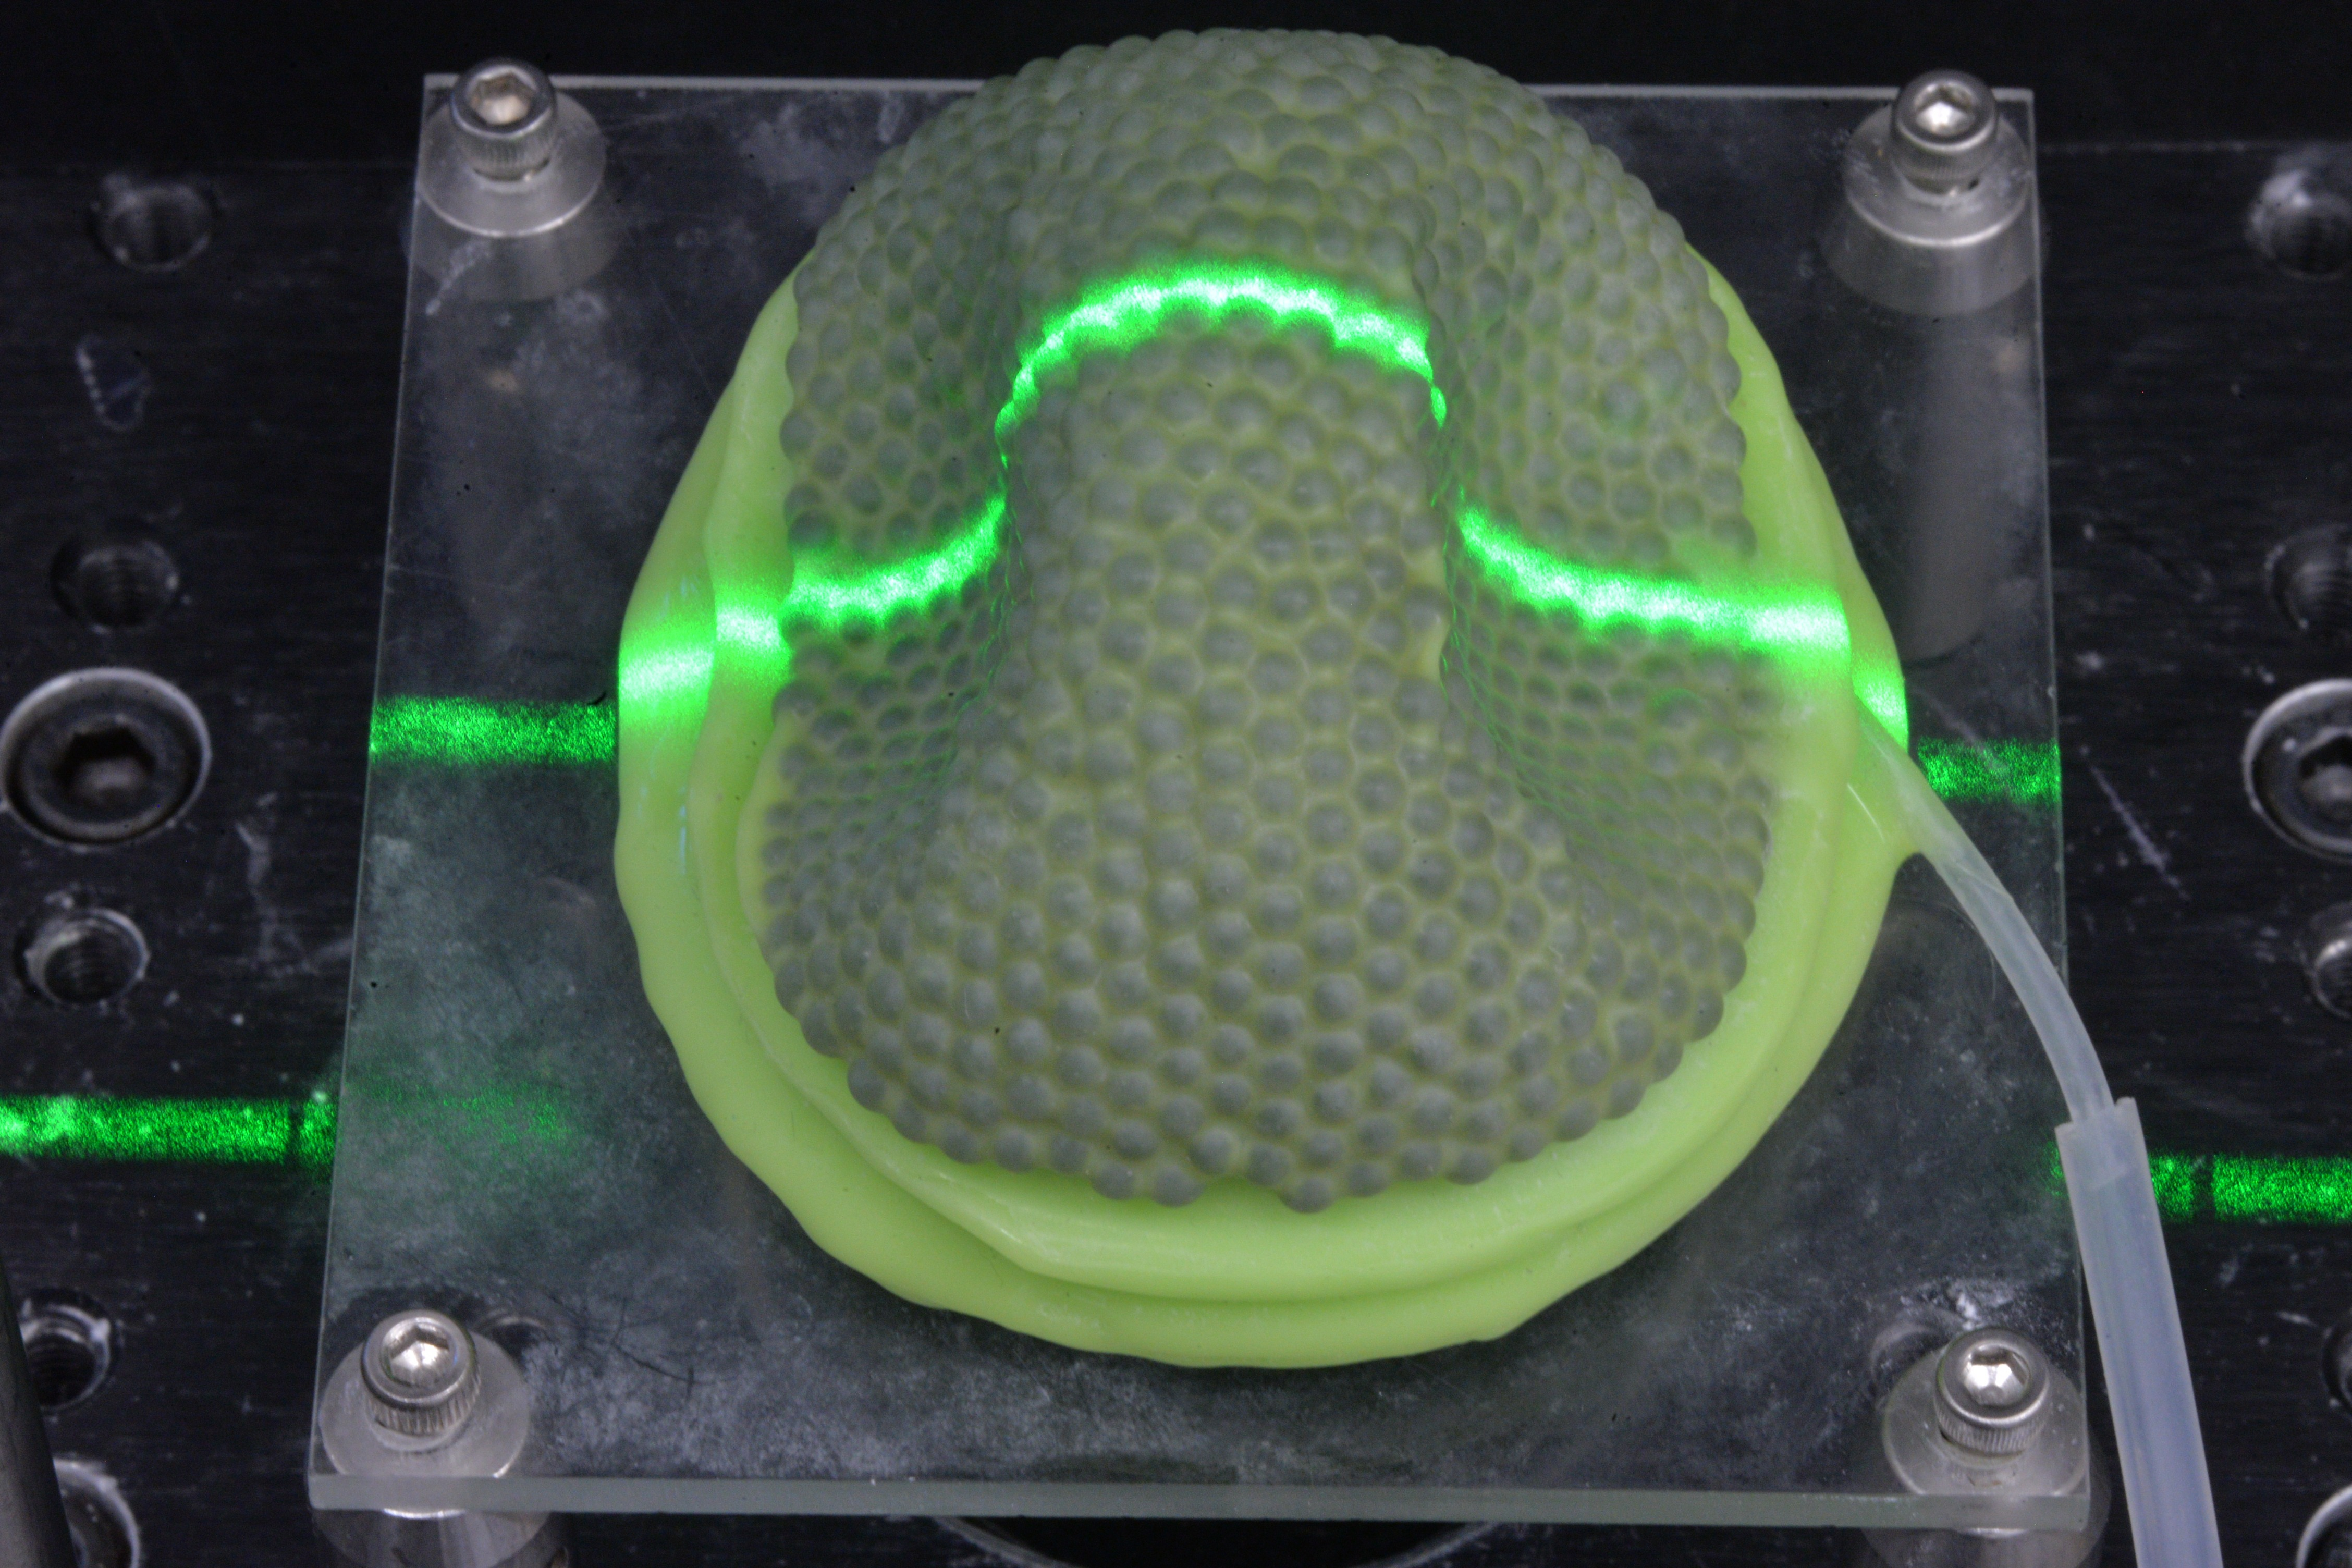
\includegraphics[width=1.5cm, trim= 110 10 90 10,clip]{indent-pinch}};
			\node[anchor=north, inner sep=.5cm] at (axis cs:6, 1.190004543) {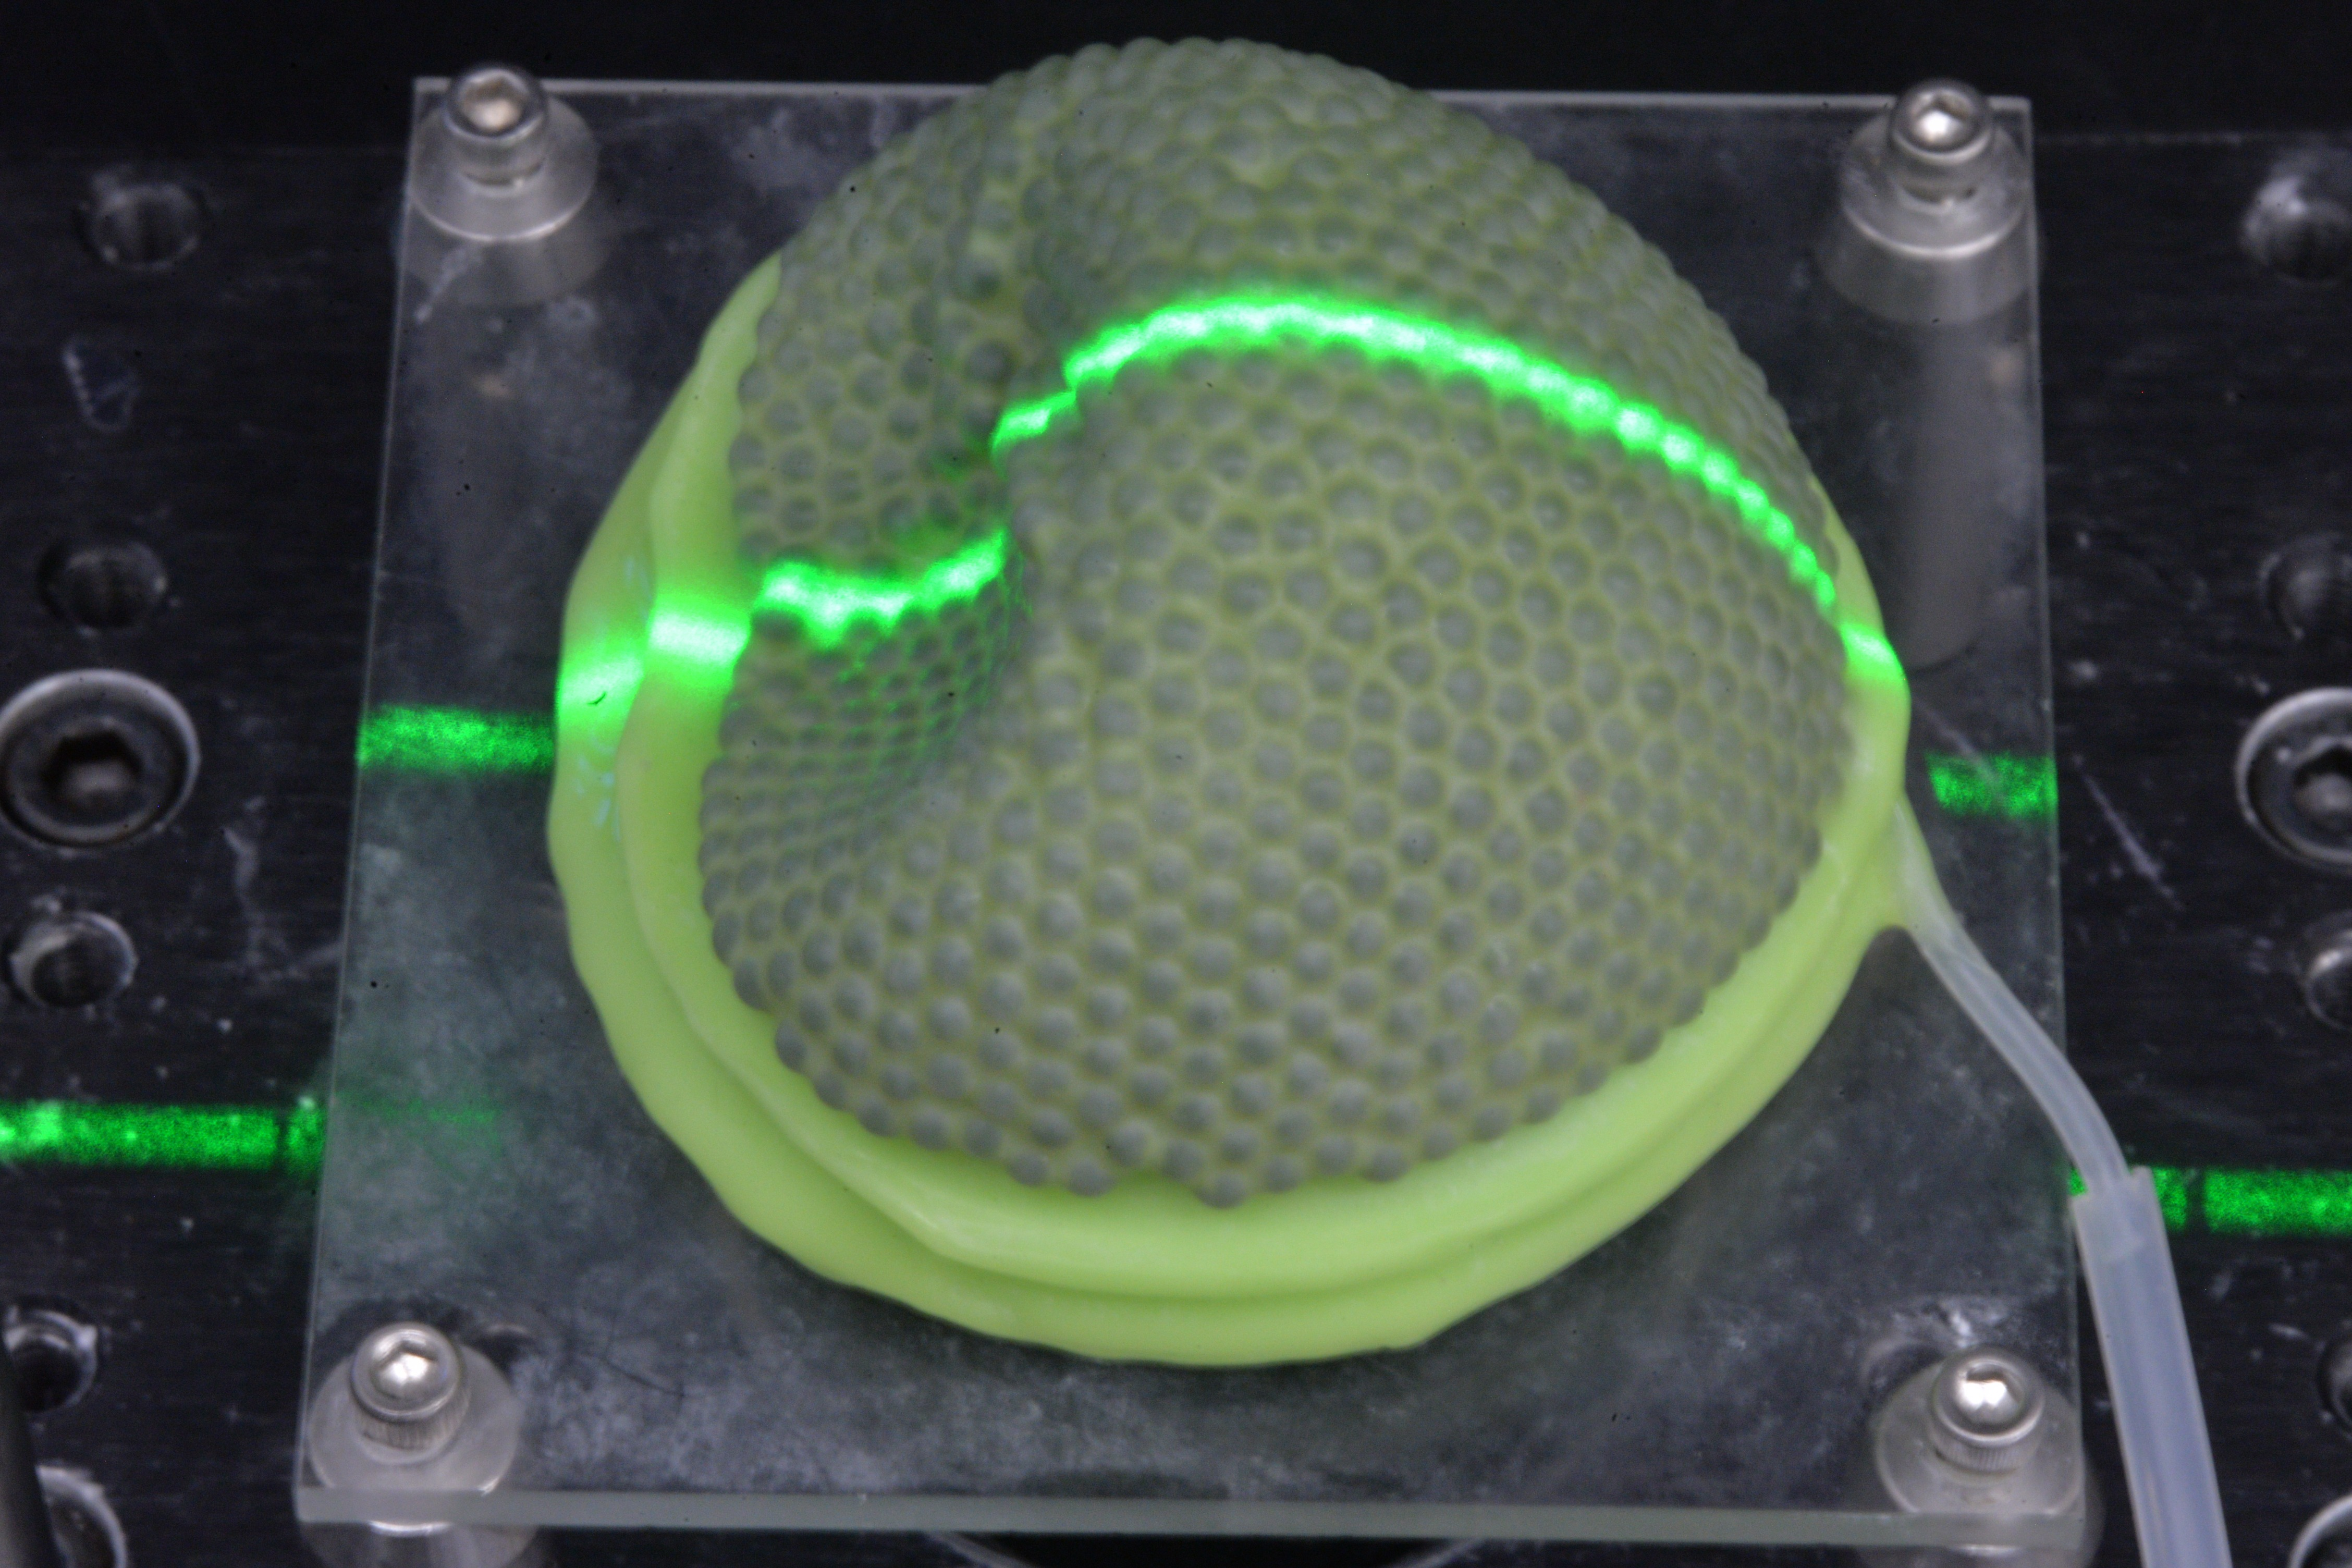
\includegraphics[width=1.5cm, trim= 110 10 90 10,clip]{indent-side}};
			\node[anchor=north, inner sep=.5cm] at (axis cs:8, 1.2964946) {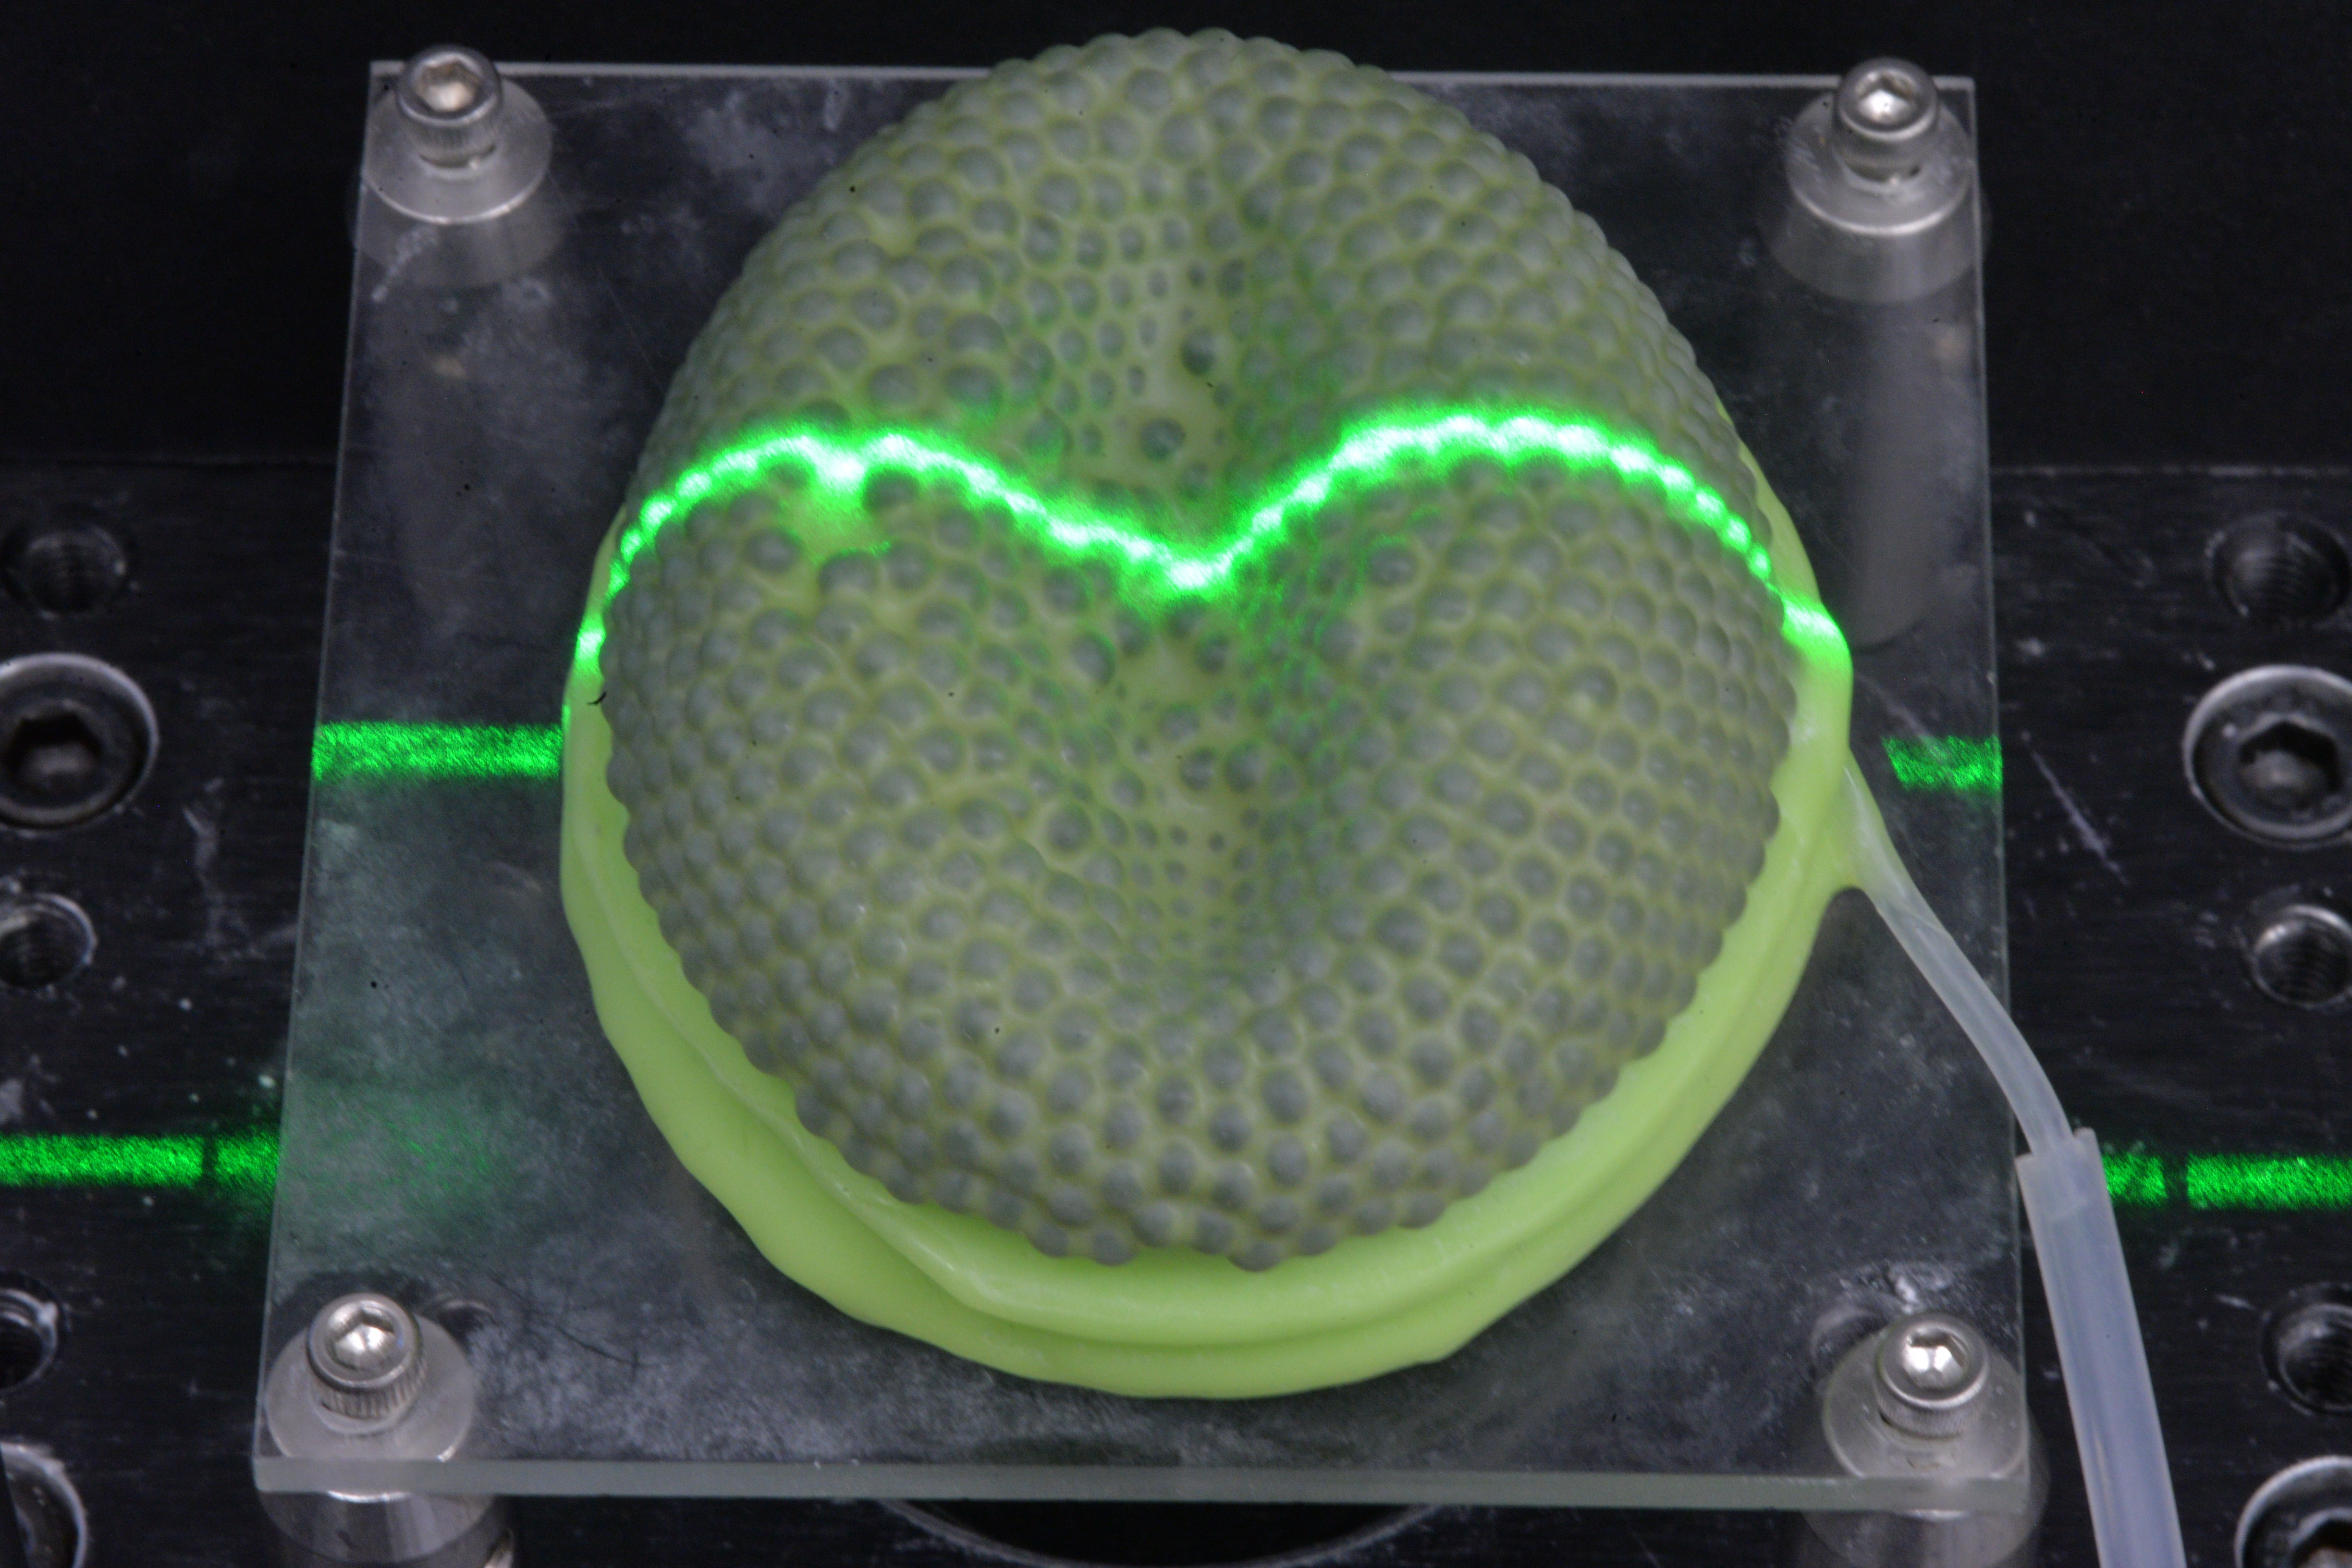
\includegraphics[width=1.5cm, trim= 100 12 100 8,clip]{indent-rod}};
			\node[anchor=north, inner sep=.5cm] at (axis cs:10, 1.522571325) {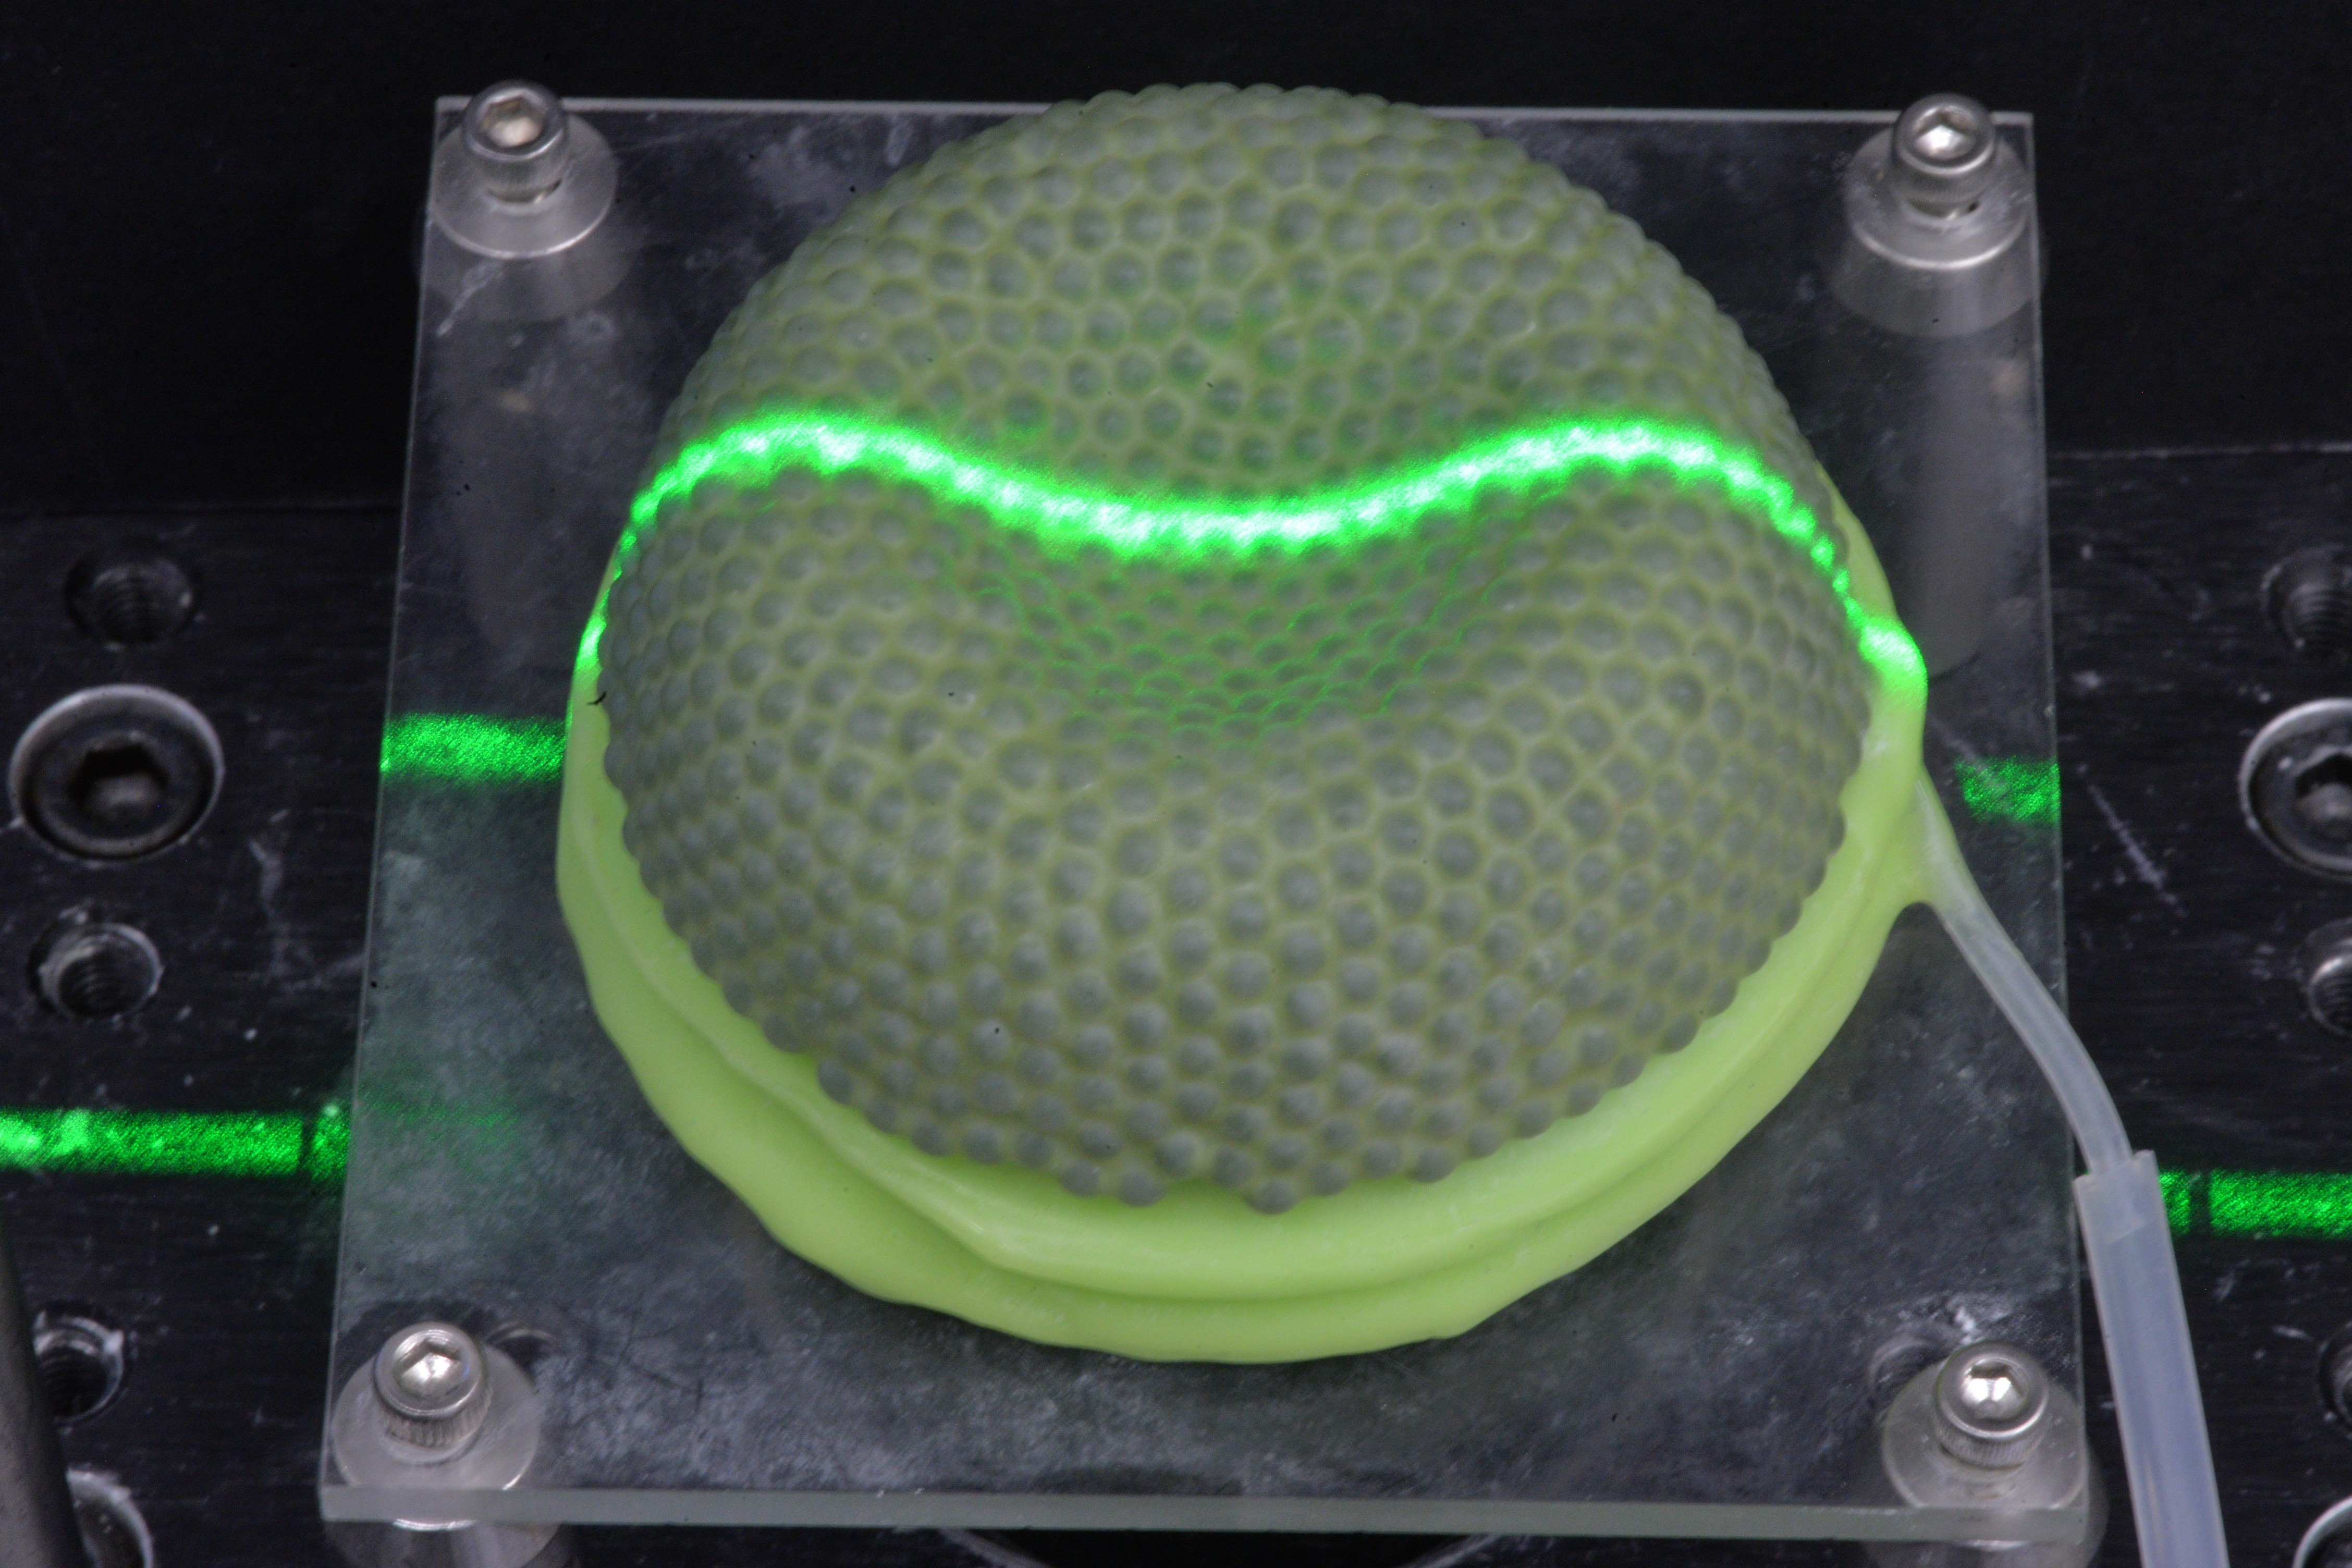
\includegraphics[width=1.5cm, trim= 110 10 90 10,clip]{indent-point}};

		\end{axis}
		
		
	\end{tikzpicture}

	
\end{document}